% Options for packages loaded elsewhere
% Options for packages loaded elsewhere
\PassOptionsToPackage{unicode}{hyperref}
\PassOptionsToPackage{hyphens}{url}
\PassOptionsToPackage{dvipsnames,svgnames,x11names}{xcolor}
%
\documentclass[
  letterpaper,
  DIV=11,
  numbers=noendperiod]{scrartcl}
\usepackage{xcolor}
\usepackage{amsmath,amssymb}
\setcounter{secnumdepth}{-\maxdimen} % remove section numbering
\usepackage{iftex}
\ifPDFTeX
  \usepackage[T1]{fontenc}
  \usepackage[utf8]{inputenc}
  \usepackage{textcomp} % provide euro and other symbols
\else % if luatex or xetex
  \usepackage{unicode-math} % this also loads fontspec
  \defaultfontfeatures{Scale=MatchLowercase}
  \defaultfontfeatures[\rmfamily]{Ligatures=TeX,Scale=1}
\fi
\usepackage{lmodern}
\ifPDFTeX\else
  % xetex/luatex font selection
\fi
% Use upquote if available, for straight quotes in verbatim environments
\IfFileExists{upquote.sty}{\usepackage{upquote}}{}
\IfFileExists{microtype.sty}{% use microtype if available
  \usepackage[]{microtype}
  \UseMicrotypeSet[protrusion]{basicmath} % disable protrusion for tt fonts
}{}
\makeatletter
\@ifundefined{KOMAClassName}{% if non-KOMA class
  \IfFileExists{parskip.sty}{%
    \usepackage{parskip}
  }{% else
    \setlength{\parindent}{0pt}
    \setlength{\parskip}{6pt plus 2pt minus 1pt}}
}{% if KOMA class
  \KOMAoptions{parskip=half}}
\makeatother
% Make \paragraph and \subparagraph free-standing
\makeatletter
\ifx\paragraph\undefined\else
  \let\oldparagraph\paragraph
  \renewcommand{\paragraph}{
    \@ifstar
      \xxxParagraphStar
      \xxxParagraphNoStar
  }
  \newcommand{\xxxParagraphStar}[1]{\oldparagraph*{#1}\mbox{}}
  \newcommand{\xxxParagraphNoStar}[1]{\oldparagraph{#1}\mbox{}}
\fi
\ifx\subparagraph\undefined\else
  \let\oldsubparagraph\subparagraph
  \renewcommand{\subparagraph}{
    \@ifstar
      \xxxSubParagraphStar
      \xxxSubParagraphNoStar
  }
  \newcommand{\xxxSubParagraphStar}[1]{\oldsubparagraph*{#1}\mbox{}}
  \newcommand{\xxxSubParagraphNoStar}[1]{\oldsubparagraph{#1}\mbox{}}
\fi
\makeatother

\usepackage{color}
\usepackage{fancyvrb}
\newcommand{\VerbBar}{|}
\newcommand{\VERB}{\Verb[commandchars=\\\{\}]}
\DefineVerbatimEnvironment{Highlighting}{Verbatim}{commandchars=\\\{\}}
% Add ',fontsize=\small' for more characters per line
\usepackage{framed}
\definecolor{shadecolor}{RGB}{241,243,245}
\newenvironment{Shaded}{\begin{snugshade}}{\end{snugshade}}
\newcommand{\AlertTok}[1]{\textcolor[rgb]{0.68,0.00,0.00}{#1}}
\newcommand{\AnnotationTok}[1]{\textcolor[rgb]{0.37,0.37,0.37}{#1}}
\newcommand{\AttributeTok}[1]{\textcolor[rgb]{0.40,0.45,0.13}{#1}}
\newcommand{\BaseNTok}[1]{\textcolor[rgb]{0.68,0.00,0.00}{#1}}
\newcommand{\BuiltInTok}[1]{\textcolor[rgb]{0.00,0.23,0.31}{#1}}
\newcommand{\CharTok}[1]{\textcolor[rgb]{0.13,0.47,0.30}{#1}}
\newcommand{\CommentTok}[1]{\textcolor[rgb]{0.37,0.37,0.37}{#1}}
\newcommand{\CommentVarTok}[1]{\textcolor[rgb]{0.37,0.37,0.37}{\textit{#1}}}
\newcommand{\ConstantTok}[1]{\textcolor[rgb]{0.56,0.35,0.01}{#1}}
\newcommand{\ControlFlowTok}[1]{\textcolor[rgb]{0.00,0.23,0.31}{\textbf{#1}}}
\newcommand{\DataTypeTok}[1]{\textcolor[rgb]{0.68,0.00,0.00}{#1}}
\newcommand{\DecValTok}[1]{\textcolor[rgb]{0.68,0.00,0.00}{#1}}
\newcommand{\DocumentationTok}[1]{\textcolor[rgb]{0.37,0.37,0.37}{\textit{#1}}}
\newcommand{\ErrorTok}[1]{\textcolor[rgb]{0.68,0.00,0.00}{#1}}
\newcommand{\ExtensionTok}[1]{\textcolor[rgb]{0.00,0.23,0.31}{#1}}
\newcommand{\FloatTok}[1]{\textcolor[rgb]{0.68,0.00,0.00}{#1}}
\newcommand{\FunctionTok}[1]{\textcolor[rgb]{0.28,0.35,0.67}{#1}}
\newcommand{\ImportTok}[1]{\textcolor[rgb]{0.00,0.46,0.62}{#1}}
\newcommand{\InformationTok}[1]{\textcolor[rgb]{0.37,0.37,0.37}{#1}}
\newcommand{\KeywordTok}[1]{\textcolor[rgb]{0.00,0.23,0.31}{\textbf{#1}}}
\newcommand{\NormalTok}[1]{\textcolor[rgb]{0.00,0.23,0.31}{#1}}
\newcommand{\OperatorTok}[1]{\textcolor[rgb]{0.37,0.37,0.37}{#1}}
\newcommand{\OtherTok}[1]{\textcolor[rgb]{0.00,0.23,0.31}{#1}}
\newcommand{\PreprocessorTok}[1]{\textcolor[rgb]{0.68,0.00,0.00}{#1}}
\newcommand{\RegionMarkerTok}[1]{\textcolor[rgb]{0.00,0.23,0.31}{#1}}
\newcommand{\SpecialCharTok}[1]{\textcolor[rgb]{0.37,0.37,0.37}{#1}}
\newcommand{\SpecialStringTok}[1]{\textcolor[rgb]{0.13,0.47,0.30}{#1}}
\newcommand{\StringTok}[1]{\textcolor[rgb]{0.13,0.47,0.30}{#1}}
\newcommand{\VariableTok}[1]{\textcolor[rgb]{0.07,0.07,0.07}{#1}}
\newcommand{\VerbatimStringTok}[1]{\textcolor[rgb]{0.13,0.47,0.30}{#1}}
\newcommand{\WarningTok}[1]{\textcolor[rgb]{0.37,0.37,0.37}{\textit{#1}}}

\usepackage{longtable,booktabs,array}
\usepackage{calc} % for calculating minipage widths
% Correct order of tables after \paragraph or \subparagraph
\usepackage{etoolbox}
\makeatletter
\patchcmd\longtable{\par}{\if@noskipsec\mbox{}\fi\par}{}{}
\makeatother
% Allow footnotes in longtable head/foot
\IfFileExists{footnotehyper.sty}{\usepackage{footnotehyper}}{\usepackage{footnote}}
\makesavenoteenv{longtable}
\usepackage{graphicx}
\makeatletter
\newsavebox\pandoc@box
\newcommand*\pandocbounded[1]{% scales image to fit in text height/width
  \sbox\pandoc@box{#1}%
  \Gscale@div\@tempa{\textheight}{\dimexpr\ht\pandoc@box+\dp\pandoc@box\relax}%
  \Gscale@div\@tempb{\linewidth}{\wd\pandoc@box}%
  \ifdim\@tempb\p@<\@tempa\p@\let\@tempa\@tempb\fi% select the smaller of both
  \ifdim\@tempa\p@<\p@\scalebox{\@tempa}{\usebox\pandoc@box}%
  \else\usebox{\pandoc@box}%
  \fi%
}
% Set default figure placement to htbp
\def\fps@figure{htbp}
\makeatother





\setlength{\emergencystretch}{3em} % prevent overfull lines

\providecommand{\tightlist}{%
  \setlength{\itemsep}{0pt}\setlength{\parskip}{0pt}}



 


\KOMAoption{captions}{tableheading}
\makeatletter
\@ifpackageloaded{tcolorbox}{}{\usepackage[skins,breakable]{tcolorbox}}
\@ifpackageloaded{fontawesome5}{}{\usepackage{fontawesome5}}
\definecolor{quarto-callout-color}{HTML}{909090}
\definecolor{quarto-callout-note-color}{HTML}{0758E5}
\definecolor{quarto-callout-important-color}{HTML}{CC1914}
\definecolor{quarto-callout-warning-color}{HTML}{EB9113}
\definecolor{quarto-callout-tip-color}{HTML}{00A047}
\definecolor{quarto-callout-caution-color}{HTML}{FC5300}
\definecolor{quarto-callout-color-frame}{HTML}{acacac}
\definecolor{quarto-callout-note-color-frame}{HTML}{4582ec}
\definecolor{quarto-callout-important-color-frame}{HTML}{d9534f}
\definecolor{quarto-callout-warning-color-frame}{HTML}{f0ad4e}
\definecolor{quarto-callout-tip-color-frame}{HTML}{02b875}
\definecolor{quarto-callout-caution-color-frame}{HTML}{fd7e14}
\makeatother
\makeatletter
\@ifpackageloaded{caption}{}{\usepackage{caption}}
\AtBeginDocument{%
\ifdefined\contentsname
  \renewcommand*\contentsname{Table of contents}
\else
  \newcommand\contentsname{Table of contents}
\fi
\ifdefined\listfigurename
  \renewcommand*\listfigurename{List of Figures}
\else
  \newcommand\listfigurename{List of Figures}
\fi
\ifdefined\listtablename
  \renewcommand*\listtablename{List of Tables}
\else
  \newcommand\listtablename{List of Tables}
\fi
\ifdefined\figurename
  \renewcommand*\figurename{Figure}
\else
  \newcommand\figurename{Figure}
\fi
\ifdefined\tablename
  \renewcommand*\tablename{Table}
\else
  \newcommand\tablename{Table}
\fi
}
\@ifpackageloaded{float}{}{\usepackage{float}}
\floatstyle{ruled}
\@ifundefined{c@chapter}{\newfloat{codelisting}{h}{lop}}{\newfloat{codelisting}{h}{lop}[chapter]}
\floatname{codelisting}{Listing}
\newcommand*\listoflistings{\listof{codelisting}{List of Listings}}
\makeatother
\makeatletter
\makeatother
\makeatletter
\@ifpackageloaded{caption}{}{\usepackage{caption}}
\@ifpackageloaded{subcaption}{}{\usepackage{subcaption}}
\makeatother
\usepackage{bookmark}
\IfFileExists{xurl.sty}{\usepackage{xurl}}{} % add URL line breaks if available
\urlstyle{same}
\hypersetup{
  pdftitle={Econometrics},
  pdfauthor={Lucia Sauer},
  colorlinks=true,
  linkcolor={blue},
  filecolor={Maroon},
  citecolor={Blue},
  urlcolor={Blue},
  pdfcreator={LaTeX via pandoc}}


\title{Econometrics}
\usepackage{etoolbox}
\makeatletter
\providecommand{\subtitle}[1]{% add subtitle to \maketitle
  \apptocmd{\@title}{\par {\large #1 \par}}{}{}
}
\makeatother
\subtitle{{TA Session 4}}
\author{Lucia Sauer}
\date{2025-10-15}
\begin{document}
\maketitle


\subsection{Overview}\label{overview}

\begin{itemize}
\tightlist
\item
  Global Hypothesis Testing
\item
  Multiple Hypothesis Testing
\item
  Monte Carlo Simulations
\end{itemize}

\begin{center}\rule{0.5\linewidth}{0.5pt}\end{center}

Let's start by running the following regression:

\[\begin{equation}
\begin{split}
\texttt{colGPA}_i &= \beta_1 + \beta_2\texttt{hsGPA}_i + \beta_3\texttt{job19}_i + \beta_4\texttt{job20}_i \\
&\quad + \beta_5\texttt{skipped}_i + \beta_6\texttt{bgfriend}_i + \beta_7\texttt{alcohol}_i + \varepsilon_i
\end{split}
\end{equation}\]

where:

\begin{itemize}
\tightlist
\item
  \(\texttt{colGPA}\): college GPA
\item
  \(\texttt{hsGPA}\): high school GPA
\item
  \(\texttt{job19}\): =1 if job \textless= 19 hours
\item
  \(\texttt{job20}\): =1 if job \textgreater= 20 hours
\item
  \(\texttt{skipped}\): avg lectures missed per week
\item
  \(\texttt{bgfriend}\): has a boyfriend/girlfriend (1=yes, 0=no)
\item
  \(\texttt{alcohol}\): avg \# days per week drink alcohol
\end{itemize}

\begin{center}\rule{0.5\linewidth}{0.5pt}\end{center}

\begin{Shaded}
\begin{Highlighting}[]
\NormalTok{bcuse gpa1, }\KeywordTok{clear}
\KeywordTok{regress}\NormalTok{ colgpa hsGPA job19 job20 skipped bgfriend alcohol}
\end{Highlighting}
\end{Shaded}

\begin{tcolorbox}[enhanced jigsaw, rightrule=.15mm, leftrule=.75mm, colback=white, left=2mm, colframe=quarto-callout-caution-color-frame, coltitle=black, opacitybacktitle=0.6, bottomrule=.15mm, toprule=.15mm, colbacktitle=quarto-callout-caution-color!10!white, breakable, titlerule=0mm, opacityback=0, toptitle=1mm, bottomtitle=1mm, title={Global Hypothesis Testing}, arc=.35mm]

What is testing the F value present in the regression output?

\end{tcolorbox}

\begin{center}\rule{0.5\linewidth}{0.5pt}\end{center}

\subsection{Global Hypothesis Testing}\label{global-hypothesis-testing}

We want to test whether our regression model adds explanatory power
beyond the mean.

\begin{tcolorbox}[enhanced jigsaw, rightrule=.15mm, leftrule=.75mm, colback=white, left=2mm, colframe=quarto-callout-warning-color-frame, coltitle=black, opacitybacktitle=0.6, bottomrule=.15mm, toprule=.15mm, colbacktitle=quarto-callout-warning-color!10!white, breakable, titlerule=0mm, opacityback=0, toptitle=1mm, bottomtitle=1mm, title={Exercise}, arc=.35mm]

\begin{enumerate}
\def\labelenumi{\arabic{enumi}.}
\tightlist
\item
  Indicate \textbf{null and alternative hypotheses}.
\item
  Write the expression of the \textbf{F-test statistic} used for this
  test, and its assumed distribution.
\item
  Run the restricted model, compute the RSSE (restricted model), SSE
  (unrestricted model) and F-statistic.
\item
  Find the critical value of the F-distribution and compute the p-value.
\end{enumerate}

\end{tcolorbox}

\begin{center}\rule{0.5\linewidth}{0.5pt}\end{center}

\subsubsection{\texorpdfstring{1. Indicate \textbf{null and alternative
hypotheses}.}{1. Indicate null and alternative hypotheses.}}\label{indicate-null-and-alternative-hypotheses.}

\begin{center}\rule{0.5\linewidth}{0.5pt}\end{center}

\begin{center}\rule{0.5\linewidth}{0.5pt}\end{center}

\subsubsection{\texorpdfstring{2. \textbf{F-test
statistic}}{2. F-test statistic}}\label{f-test-statistic}

\begin{center}\rule{0.5\linewidth}{0.5pt}\end{center}

\begin{center}\rule{0.5\linewidth}{0.5pt}\end{center}

\subsubsection{3. RSSE and SSE}\label{rsse-and-sse}

\begin{center}\rule{0.5\linewidth}{0.5pt}\end{center}

\begin{center}\rule{0.5\linewidth}{0.5pt}\end{center}

\subsubsection{4. Critical value and
p-value}\label{critical-value-and-p-value}

\begin{center}\rule{0.5\linewidth}{0.5pt}\end{center}

\begin{center}\rule{0.5\linewidth}{0.5pt}\end{center}

\subsubsection{5. Draw the p-value and the critical
value}\label{draw-the-p-value-and-the-critical-value}

\begin{center}\rule{0.5\linewidth}{0.5pt}\end{center}

\begin{center}\rule{0.5\linewidth}{0.5pt}\end{center}

\subsection{Multiple Hypothesis
Testing}\label{multiple-hypothesis-testing}

Consider testing whether job19 and job20 are jointly significant at
\(\alpha=0.05\):

\begin{tcolorbox}[enhanced jigsaw, rightrule=.15mm, leftrule=.75mm, colback=white, left=2mm, colframe=quarto-callout-warning-color-frame, coltitle=black, opacitybacktitle=0.6, bottomrule=.15mm, toprule=.15mm, colbacktitle=quarto-callout-warning-color!10!white, breakable, titlerule=0mm, opacityback=0, toptitle=1mm, bottomtitle=1mm, title={Exercise}, arc=.35mm]

\begin{enumerate}
\def\labelenumi{\arabic{enumi}.}
\tightlist
\item
  Indicate \textbf{null and alternative hypotheses}.
\item
  Write the expression of the \textbf{F-test statistic} used for this
  test, and its assumed distribution.
\item
  Run the restricted model, compute the RSSE (restricted model), SSE
  (unrestricted model) and F-statistic.
\item
  Find the critical value of the F-distribution and compute the p-value.
\item
  Draw the p-value and the critical value.
\item
  Compare the results with the ones obtained in Stata.
\end{enumerate}

\end{tcolorbox}

\begin{center}\rule{0.5\linewidth}{0.5pt}\end{center}

\subsubsection{\texorpdfstring{1. Indicate \textbf{null and alternative
hypotheses}.}{1. Indicate null and alternative hypotheses.}}\label{indicate-null-and-alternative-hypotheses.-1}

\begin{center}\rule{0.5\linewidth}{0.5pt}\end{center}

\begin{center}\rule{0.5\linewidth}{0.5pt}\end{center}

\subsubsection{\texorpdfstring{2. \textbf{F-test
statistic}}{2. F-test statistic}}\label{f-test-statistic-1}

\begin{center}\rule{0.5\linewidth}{0.5pt}\end{center}

\begin{center}\rule{0.5\linewidth}{0.5pt}\end{center}

\subsubsection{3. RSSE and SSE}\label{rsse-and-sse-1}

\begin{center}\rule{0.5\linewidth}{0.5pt}\end{center}

\begin{center}\rule{0.5\linewidth}{0.5pt}\end{center}

\begin{center}\rule{0.5\linewidth}{0.5pt}\end{center}

\subsubsection{4. Critical value and
p-value}\label{critical-value-and-p-value-1}

\begin{center}\rule{0.5\linewidth}{0.5pt}\end{center}

\begin{center}\rule{0.5\linewidth}{0.5pt}\end{center}

\subsubsection{5. Draw the p-value and the critical
value}\label{draw-the-p-value-and-the-critical-value-1}

\begin{center}\rule{0.5\linewidth}{0.5pt}\end{center}

\begin{center}\rule{0.5\linewidth}{0.5pt}\end{center}

\subsection{Monte Carlo Simulations}\label{monte-carlo-simulations}

Monte Carlo Casino

\begin{center}\rule{0.5\linewidth}{0.5pt}\end{center}

\begin{tcolorbox}[enhanced jigsaw, rightrule=.15mm, leftrule=.75mm, colback=white, left=2mm, colframe=quarto-callout-tip-color-frame, coltitle=black, opacitybacktitle=0.6, bottomrule=.15mm, toprule=.15mm, colbacktitle=quarto-callout-tip-color!10!white, breakable, titlerule=0mm, opacityback=0, toptitle=1mm, bottomtitle=1mm, title=\textcolor{quarto-callout-tip-color}{\faLightbulb}\hspace{0.5em}{Monte Carlo: a lab for estimators}, arc=.35mm]

\textbf{Workflow}

\begin{enumerate}
\def\labelenumi{\arabic{enumi}.}
\tightlist
\item
  \textbf{Specify a known DGP} (the ``true'' model).
\item
  \textbf{Generate} many random samples from it.
\item
  \textbf{Estimate} the coefficients repeatedly.
\item
  \textbf{Observe} the estimator's behavior across replications:

  \begin{itemize}
  \tightlist
  \item
    mean (\emph{bias})
  \item
    spread (\emph{variance})
  \item
    shape (\emph{sampling distribution})
  \end{itemize}
\end{enumerate}

\end{tcolorbox}

\begin{center}\rule{0.5\linewidth}{0.5pt}\end{center}

\subsubsection{Data-Generating Process
(DGP)}\label{data-generating-process-dgp}

We will generate \(m=10000\) samples of size \(n=100\) from the
following DGP:

\begin{tcolorbox}[enhanced jigsaw, rightrule=.15mm, leftrule=.75mm, colback=white, left=2mm, colframe=quarto-callout-tip-color-frame, coltitle=black, opacitybacktitle=0.6, bottomrule=.15mm, toprule=.15mm, colbacktitle=quarto-callout-tip-color!10!white, breakable, titlerule=0mm, opacityback=0, toptitle=1mm, bottomtitle=1mm, title={DGP}, arc=.35mm]

\[
y_i = 4 + 2x_{i2} + 2x_{i3} + \varepsilon_i 
\]

\[\varepsilon_i \,|\, X_i \sim \text{i.i.d. } N(0,32)\]

\[
x_{i2} \sim U[0,40], \quad
x_{i3} = x_{i2} + v_i, \; v_i \sim N(0, 16)
\]

\end{tcolorbox}

\begin{center}\rule{0.5\linewidth}{0.5pt}\end{center}

\subsubsection{Function in Python}\label{function-in-python}

Let's create a function to analyze the behavior of \(\hat{\beta}_2\):

\begin{Shaded}
\begin{Highlighting}[]
\KeywordTok{def}\NormalTok{ simulate\_betas(n}\OperatorTok{=}\DecValTok{100}\NormalTok{, sigma\_eps}\OperatorTok{=}\DecValTok{32}\NormalTok{, sigma\_v}\OperatorTok{=}\DecValTok{16}\NormalTok{, reps}\OperatorTok{=}\DecValTok{10000}\NormalTok{, conditional}\OperatorTok{=}\VariableTok{False}\NormalTok{):}
    \CommentTok{"""}
\CommentTok{    Monte Carlo simulation of β₂ from y = 4 + 2x₂ + 2x₃ + ε.}
\CommentTok{    """}
\NormalTok{    betas }\OperatorTok{=}\NormalTok{ []}
    
    \CommentTok{\# For conditional distribution: fix X once}
    \ControlFlowTok{if}\NormalTok{ conditional:}
\NormalTok{        x2\_fixed }\OperatorTok{=}\NormalTok{ np.random.uniform(}\DecValTok{0}\NormalTok{, }\DecValTok{40}\NormalTok{, n)}
\NormalTok{        v\_fixed  }\OperatorTok{=}\NormalTok{ np.random.normal(}\DecValTok{0}\NormalTok{, sigma\_v, n)}
\NormalTok{        x3\_fixed }\OperatorTok{=}\NormalTok{ x2\_fixed }\OperatorTok{+}\NormalTok{ v\_fixed}
    
    \ControlFlowTok{for}\NormalTok{ \_ }\KeywordTok{in} \BuiltInTok{range}\NormalTok{(reps):}
        \ControlFlowTok{if}\NormalTok{ conditional:}
\NormalTok{            x2, x3 }\OperatorTok{=}\NormalTok{ x2\_fixed, x3\_fixed}
        \ControlFlowTok{else}\NormalTok{:}
\NormalTok{            x2 }\OperatorTok{=}\NormalTok{ np.random.uniform(}\DecValTok{0}\NormalTok{, }\DecValTok{40}\NormalTok{, n)}
\NormalTok{            v  }\OperatorTok{=}\NormalTok{ np.random.normal(}\DecValTok{0}\NormalTok{, sigma\_v, n)}
\NormalTok{            x3 }\OperatorTok{=}\NormalTok{ x2 }\OperatorTok{+}\NormalTok{ v}

\NormalTok{        eps }\OperatorTok{=}\NormalTok{ np.random.normal(}\DecValTok{0}\NormalTok{, sigma\_eps, n)}
\NormalTok{        y }\OperatorTok{=} \DecValTok{4} \OperatorTok{+} \DecValTok{2}\OperatorTok{*}\NormalTok{x2 }\OperatorTok{+} \DecValTok{2}\OperatorTok{*}\NormalTok{x3 }\OperatorTok{+}\NormalTok{ eps}

\NormalTok{        X }\OperatorTok{=}\NormalTok{ sm.add\_constant(np.column\_stack([x2, x3]))}
\NormalTok{        model }\OperatorTok{=}\NormalTok{ sm.OLS(y, X).fit()}
\NormalTok{        betas.append(model.params[}\DecValTok{1}\NormalTok{])}

    \ControlFlowTok{return}\NormalTok{ np.array(betas)}
\end{Highlighting}
\end{Shaded}

\begin{center}\rule{0.5\linewidth}{0.5pt}\end{center}

Let's run the simulation for the conditional distribution of
\(\hat{\beta}_2\):

\begin{Shaded}
\begin{Highlighting}[]
\NormalTok{betas\_base }\OperatorTok{=}\NormalTok{ simulate\_betas(n}\OperatorTok{=}\DecValTok{1000}\NormalTok{, sigma\_eps}\OperatorTok{=}\DecValTok{32}\NormalTok{, sigma\_v}\OperatorTok{=}\DecValTok{16}\NormalTok{, reps}\OperatorTok{=}\DecValTok{10000}\NormalTok{)}

\NormalTok{plt.figure(figsize}\OperatorTok{=}\NormalTok{(}\DecValTok{6}\NormalTok{,}\DecValTok{5}\NormalTok{))}
\NormalTok{sns.kdeplot(betas\_base, fill}\OperatorTok{=}\VariableTok{True}\NormalTok{, alpha}\OperatorTok{=}\FloatTok{0.5}\NormalTok{, color}\OperatorTok{=}\StringTok{"purple"}\NormalTok{, label}\OperatorTok{=}\StringTok{"Baseline"}\NormalTok{, edgecolor}\OperatorTok{=}\StringTok{"black"}\NormalTok{)}
\NormalTok{plt.axvline(}\DecValTok{2}\NormalTok{, color}\OperatorTok{=}\StringTok{"black"}\NormalTok{, ls}\OperatorTok{=}\StringTok{"{-}{-}"}\NormalTok{, label}\OperatorTok{=}\VerbatimStringTok{r"True }\DecValTok{$\textbackslash{}b}\VerbatimStringTok{eta\_2}\DecValTok{$}\VerbatimStringTok{"}\NormalTok{)}
\NormalTok{plt.title(}\VerbatimStringTok{r"}\DecValTok{$}\ErrorTok{\textbackslash{}}\VerbatimStringTok{hat\{}\DecValTok{\textbackslash{}b}\VerbatimStringTok{eta\}\_2}\DecValTok{$}\VerbatimStringTok{ sampling distribution"}\NormalTok{)}
\NormalTok{plt.xlabel(}\VerbatimStringTok{r"}\DecValTok{$}\ErrorTok{\textbackslash{}}\VerbatimStringTok{hat\{}\DecValTok{\textbackslash{}b}\VerbatimStringTok{eta\}\_2}\DecValTok{$}\VerbatimStringTok{"}\NormalTok{)}
\NormalTok{plt.show()}
\end{Highlighting}
\end{Shaded}

\begin{center}
\pandocbounded{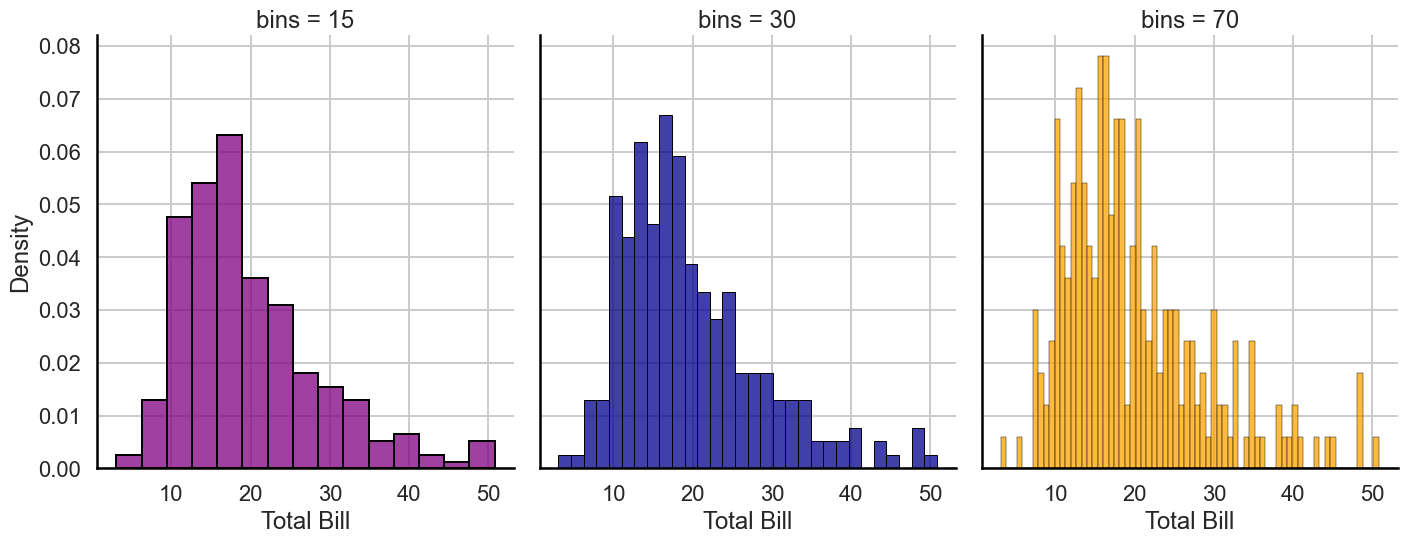
\includegraphics[keepaspectratio]{TA4_files/figure-pdf/cell-5-output-1.png}}
\end{center}

\begin{center}\rule{0.5\linewidth}{0.5pt}\end{center}

Now, let's increase \(\sigma_{\varepsilon}^2\):

\begin{Shaded}
\begin{Highlighting}[]
\NormalTok{betas\_high\_sigma }\OperatorTok{=}\NormalTok{ simulate\_betas(n}\OperatorTok{=}\DecValTok{1000}\NormalTok{, sigma\_eps}\OperatorTok{=}\DecValTok{64}\NormalTok{, sigma\_v}\OperatorTok{=}\DecValTok{16}\NormalTok{, reps}\OperatorTok{=}\DecValTok{10000}\NormalTok{)}
\NormalTok{betas\_low\_sigma }\OperatorTok{=}\NormalTok{ simulate\_betas(n}\OperatorTok{=}\DecValTok{1000}\NormalTok{, sigma\_eps}\OperatorTok{=}\DecValTok{16}\NormalTok{, sigma\_v}\OperatorTok{=}\DecValTok{16}\NormalTok{, reps}\OperatorTok{=}\DecValTok{10000}\NormalTok{)}

\NormalTok{plt.figure(figsize}\OperatorTok{=}\NormalTok{(}\DecValTok{6}\NormalTok{,}\DecValTok{5}\NormalTok{))}
\ControlFlowTok{for}\NormalTok{ sns, color, label }\KeywordTok{in} \BuiltInTok{zip}\NormalTok{([betas\_low\_sigma, betas\_base, betas\_high\_sigma], [}\VerbatimStringTok{r"}\DecValTok{$\textbackslash{}s}\VerbatimStringTok{igma\_\{}\CharTok{\textbackslash{}v}\VerbatimStringTok{arepsilon\}=16}\DecValTok{$}\VerbatimStringTok{"}\NormalTok{, }\VerbatimStringTok{r"}\DecValTok{$\textbackslash{}s}\VerbatimStringTok{igma\_\{}\CharTok{\textbackslash{}v}\VerbatimStringTok{arepsilon\}=32}\DecValTok{$}\VerbatimStringTok{"}\NormalTok{, }\VerbatimStringTok{r"}\DecValTok{$\textbackslash{}s}\VerbatimStringTok{igma\_\{}\CharTok{\textbackslash{}v}\VerbatimStringTok{arepsilon\}=64}\DecValTok{$}\VerbatimStringTok{"}\NormalTok{]):}
\NormalTok{    sns.kdeplot(sns, fill}\OperatorTok{=}\VariableTok{True}\NormalTok{, alpha}\OperatorTok{=}\FloatTok{0.5}\NormalTok{, edgecolor}\OperatorTok{=}\StringTok{"black"}\NormalTok{, color}\OperatorTok{=}\NormalTok{color, label}\OperatorTok{=}\NormalTok{label)}
\NormalTok{plt.axvline(}\DecValTok{2}\NormalTok{, color}\OperatorTok{=}\StringTok{"black"}\NormalTok{, ls}\OperatorTok{=}\StringTok{"{-}{-}"}\NormalTok{, label}\OperatorTok{=}\VerbatimStringTok{r"True }\DecValTok{$\textbackslash{}b}\VerbatimStringTok{eta\_2}\DecValTok{$}\VerbatimStringTok{"}\NormalTok{)}
\NormalTok{plt.title(}\VerbatimStringTok{r"}\DecValTok{$}\ErrorTok{\textbackslash{}}\VerbatimStringTok{hat\{}\DecValTok{\textbackslash{}b}\VerbatimStringTok{eta\}\_2}\DecValTok{$}\VerbatimStringTok{ sampling distribution"}\NormalTok{)}
\NormalTok{plt.xlabel(}\VerbatimStringTok{r"}\DecValTok{$}\ErrorTok{\textbackslash{}}\VerbatimStringTok{hat\{}\DecValTok{\textbackslash{}b}\VerbatimStringTok{eta\}\_2}\DecValTok{$}\VerbatimStringTok{"}\NormalTok{)}
\NormalTok{plt.show()}
\end{Highlighting}
\end{Shaded}

\begin{center}
\pandocbounded{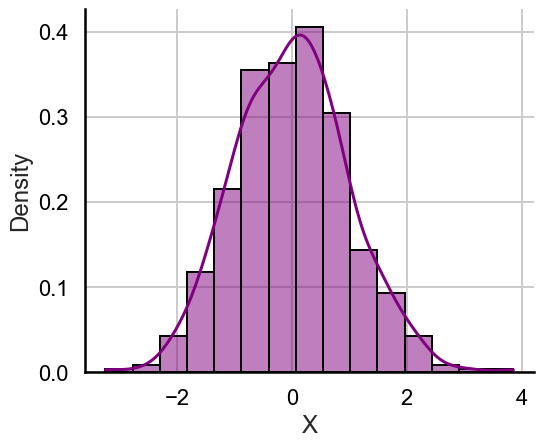
\includegraphics[keepaspectratio]{TA4_files/figure-pdf/cell-7-output-1.png}}
\end{center}

\begin{center}\rule{0.5\linewidth}{0.5pt}\end{center}

\begin{center}\rule{0.5\linewidth}{0.5pt}\end{center}

\begin{center}\rule{0.5\linewidth}{0.5pt}\end{center}

Now, let's reduce \(\sigma_{v}^2\), the collinearity between \(x_2\) and
\(x_3\):

\begin{Shaded}
\begin{Highlighting}[]
\NormalTok{betas\_high\_collinear }\OperatorTok{=}\NormalTok{ simulate\_betas(n}\OperatorTok{=}\DecValTok{1000}\NormalTok{, sigma\_eps}\OperatorTok{=}\DecValTok{32}\NormalTok{, sigma\_v}\OperatorTok{=}\DecValTok{32}\NormalTok{, reps}\OperatorTok{=}\DecValTok{10000}\NormalTok{)}
\NormalTok{betas\_low\_collinear }\OperatorTok{=}\NormalTok{ simulate\_betas(n}\OperatorTok{=}\DecValTok{1000}\NormalTok{, sigma\_eps}\OperatorTok{=}\DecValTok{32}\NormalTok{, sigma\_v}\OperatorTok{=}\DecValTok{8}\NormalTok{, reps}\OperatorTok{=}\DecValTok{10000}\NormalTok{)}

\NormalTok{plt.figure(figsize}\OperatorTok{=}\NormalTok{(}\DecValTok{6}\NormalTok{,}\DecValTok{5}\NormalTok{))}
\ControlFlowTok{for}\NormalTok{ sns, color, label }\KeywordTok{in} \BuiltInTok{zip}\NormalTok{([betas\_low\_collinear, betas\_base, betas\_high\_collinear], [}\VerbatimStringTok{r"}\DecValTok{$\textbackslash{}s}\VerbatimStringTok{igma\_\{v\}=8}\DecValTok{$}\VerbatimStringTok{"}\NormalTok{, }\VerbatimStringTok{r"}\DecValTok{$\textbackslash{}s}\VerbatimStringTok{igma\_\{v\}=16}\DecValTok{$}\VerbatimStringTok{"}\NormalTok{, }\VerbatimStringTok{r"}\DecValTok{$\textbackslash{}s}\VerbatimStringTok{igma\_\{v\}=32}\DecValTok{$}\VerbatimStringTok{"}\NormalTok{]):}
\NormalTok{    sns.kdeplot(sns, fill}\OperatorTok{=}\VariableTok{True}\NormalTok{, alpha}\OperatorTok{=}\FloatTok{0.5}\NormalTok{, edgecolor}\OperatorTok{=}\StringTok{"black"}\NormalTok{, color}\OperatorTok{=}\NormalTok{color, label}\OperatorTok{=}\NormalTok{label)}
\NormalTok{plt.axvline(}\DecValTok{2}\NormalTok{, color}\OperatorTok{=}\StringTok{"black"}\NormalTok{, ls}\OperatorTok{=}\StringTok{"{-}{-}"}\NormalTok{, label}\OperatorTok{=}\VerbatimStringTok{r"True }\DecValTok{$\textbackslash{}b}\VerbatimStringTok{eta\_2}\DecValTok{$}\VerbatimStringTok{"}\NormalTok{)}
\NormalTok{plt.title(}\VerbatimStringTok{r"}\DecValTok{$}\ErrorTok{\textbackslash{}}\VerbatimStringTok{hat\{}\DecValTok{\textbackslash{}b}\VerbatimStringTok{eta\}\_2}\DecValTok{$}\VerbatimStringTok{ sampling distribution"}\NormalTok{)}
\NormalTok{plt.xlabel(}\VerbatimStringTok{r"}\DecValTok{$}\ErrorTok{\textbackslash{}}\VerbatimStringTok{hat\{}\DecValTok{\textbackslash{}b}\VerbatimStringTok{eta\}\_2}\DecValTok{$}\VerbatimStringTok{"}\NormalTok{)}
\NormalTok{plt.show()}
\end{Highlighting}
\end{Shaded}

\begin{center}
\pandocbounded{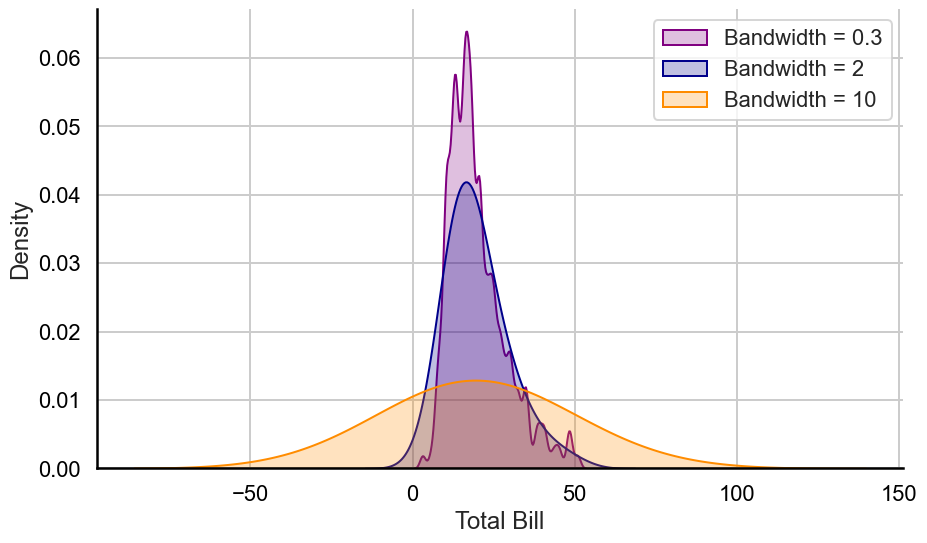
\includegraphics[keepaspectratio]{TA4_files/figure-pdf/cell-9-output-1.png}}
\end{center}

\begin{center}\rule{0.5\linewidth}{0.5pt}\end{center}

\begin{center}\rule{0.5\linewidth}{0.5pt}\end{center}

Increasing the sample size \(n\):

\begin{Shaded}
\begin{Highlighting}[]
\NormalTok{betas\_large\_sample }\OperatorTok{=}\NormalTok{ simulate\_betas(n}\OperatorTok{=}\DecValTok{10000}\NormalTok{)}
\NormalTok{betas\_small\_sample }\OperatorTok{=}\NormalTok{ simulate\_betas(n}\OperatorTok{=}\DecValTok{100}\NormalTok{)}


\NormalTok{plt.figure(figsize}\OperatorTok{=}\NormalTok{(}\DecValTok{6}\NormalTok{,}\DecValTok{5}\NormalTok{))}
\ControlFlowTok{for}\NormalTok{ sns, color, label }\KeywordTok{in} \BuiltInTok{zip}\NormalTok{([betas\_small\_sample, betas\_base, betas\_large\_sample], [}\VerbatimStringTok{r"}\DecValTok{$}\VerbatimStringTok{n=100}\DecValTok{$}\VerbatimStringTok{"}\NormalTok{, }\VerbatimStringTok{r"}\DecValTok{$}\VerbatimStringTok{n=1000}\DecValTok{$}\VerbatimStringTok{"}\NormalTok{, }\VerbatimStringTok{r"}\DecValTok{$}\VerbatimStringTok{n=10000}\DecValTok{$}\VerbatimStringTok{"}\NormalTok{]):}
\NormalTok{    sns.kdeplot(sns, fill}\OperatorTok{=}\VariableTok{True}\NormalTok{, alpha}\OperatorTok{=}\FloatTok{0.5}\NormalTok{, edgecolor}\OperatorTok{=}\StringTok{"black"}\NormalTok{, color}\OperatorTok{=}\NormalTok{color, label}\OperatorTok{=}\NormalTok{label)}
\NormalTok{plt.axvline(}\DecValTok{2}\NormalTok{, color}\OperatorTok{=}\StringTok{"black"}\NormalTok{, ls}\OperatorTok{=}\StringTok{"{-}{-}"}\NormalTok{, label}\OperatorTok{=}\VerbatimStringTok{r"True }\DecValTok{$\textbackslash{}b}\VerbatimStringTok{eta\_2}\DecValTok{$}\VerbatimStringTok{"}\NormalTok{)}
\NormalTok{plt.title(}\VerbatimStringTok{r"}\DecValTok{$}\ErrorTok{\textbackslash{}}\VerbatimStringTok{hat\{}\DecValTok{\textbackslash{}b}\VerbatimStringTok{eta\}\_2}\DecValTok{$}\VerbatimStringTok{ sampling distribution"}\NormalTok{)}
\NormalTok{plt.xlabel(}\VerbatimStringTok{r"}\DecValTok{$}\ErrorTok{\textbackslash{}}\VerbatimStringTok{hat\{}\DecValTok{\textbackslash{}b}\VerbatimStringTok{eta\}\_2}\DecValTok{$}\VerbatimStringTok{"}\NormalTok{)}
\NormalTok{plt.show()}
\end{Highlighting}
\end{Shaded}

\begin{center}
\pandocbounded{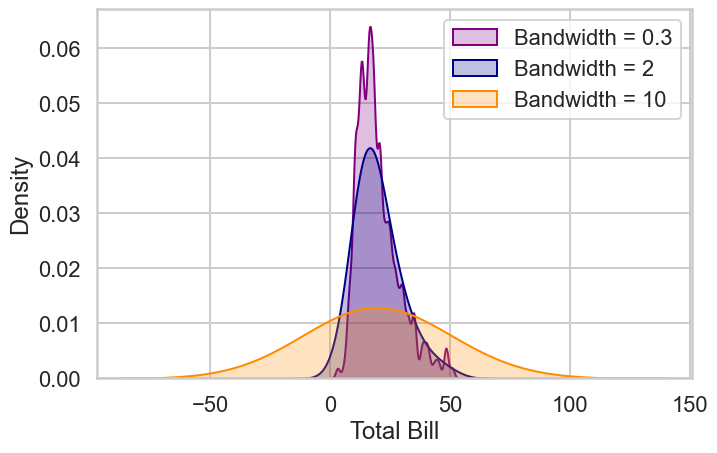
\includegraphics[keepaspectratio]{TA4_files/figure-pdf/cell-11-output-1.png}}
\end{center}

\begin{center}\rule{0.5\linewidth}{0.5pt}\end{center}

\begin{center}\rule{0.5\linewidth}{0.5pt}\end{center}

Now, running the simulation for the unconditional distribution of
\(\hat{\beta}_2\):

\begin{Shaded}
\begin{Highlighting}[]
\NormalTok{betas\_base\_cond }\OperatorTok{=}\NormalTok{ simulate\_betas()}
\NormalTok{betas\_base\_uncond }\OperatorTok{=}\NormalTok{ simulate\_betas(conditional}\OperatorTok{=}\VariableTok{True}\NormalTok{)}


\NormalTok{plt.figure(figsize}\OperatorTok{=}\NormalTok{(}\DecValTok{6}\NormalTok{,}\DecValTok{5}\NormalTok{))}
\ControlFlowTok{for}\NormalTok{ sns, color, label }\KeywordTok{in} \BuiltInTok{zip}\NormalTok{([betas\_base\_uncond, betas\_base\_cond], [}\VerbatimStringTok{r"}\DecValTok{$}\VerbatimStringTok{Conditioned on X}\DecValTok{$}\VerbatimStringTok{"}\NormalTok{, }\VerbatimStringTok{r"}\DecValTok{$}\VerbatimStringTok{Unconditioned on X}\DecValTok{$}\VerbatimStringTok{"}\NormalTok{]):}
\NormalTok{    sns.kdeplot(sns, fill}\OperatorTok{=}\VariableTok{True}\NormalTok{, alpha}\OperatorTok{=}\FloatTok{0.5}\NormalTok{, edgecolor}\OperatorTok{=}\StringTok{"black"}\NormalTok{, color}\OperatorTok{=}\NormalTok{color, label}\OperatorTok{=}\NormalTok{label)}
\NormalTok{plt.axvline(}\DecValTok{2}\NormalTok{, color}\OperatorTok{=}\StringTok{"black"}\NormalTok{, ls}\OperatorTok{=}\StringTok{"{-}{-}"}\NormalTok{, label}\OperatorTok{=}\VerbatimStringTok{r"True }\DecValTok{$\textbackslash{}b}\VerbatimStringTok{eta\_2}\DecValTok{$}\VerbatimStringTok{"}\NormalTok{)}
\NormalTok{plt.title(}\VerbatimStringTok{r"}\DecValTok{$}\ErrorTok{\textbackslash{}}\VerbatimStringTok{hat\{}\DecValTok{\textbackslash{}b}\VerbatimStringTok{eta\}\_2}\DecValTok{$}\VerbatimStringTok{ sampling distribution"}\NormalTok{)}
\NormalTok{plt.xlabel(}\VerbatimStringTok{r"}\DecValTok{$}\ErrorTok{\textbackslash{}}\VerbatimStringTok{hat\{}\DecValTok{\textbackslash{}b}\VerbatimStringTok{eta\}\_2}\DecValTok{$}\VerbatimStringTok{"}\NormalTok{)}
\NormalTok{plt.show()}
\end{Highlighting}
\end{Shaded}

\begin{center}
\pandocbounded{\includegraphics[keepaspectratio]{TA4_files/figure-pdf/cell-13-output-1.png}}
\end{center}

\begin{center}\rule{0.5\linewidth}{0.5pt}\end{center}

\begin{center}\rule{0.5\linewidth}{0.5pt}\end{center}




\end{document}
